\documentclass[11pt,ngerman]{article}
\usepackage[utf8]{inputenc}
%?
\linespread{1.0}
\setlength{\parskip}{0.7em}
\setlength{\baselineskip}{0.2cm}
\setlength{\parindent}{0em}
\usepackage[a4paper,left=2cm,right=2cm,top=2cm,bottom=2cm,bindingoffset=5mm]{geometry}
%?
\usepackage{hyperref}
\usepackage{booktabs}
\usepackage{graphicx}

\begin{document}
\title{Summary Visual Analytics}
\author{John}
\maketitle

\tableofcontents
\newpage

\section{Introduction}
\begin{itemize}
	\item Visual Analytics is the science of analytical
reasoning facilitated by interactive visual interfaces.
	\item An integrated combination of data analytics and
interactive visual exploration.
	\item aims at supporting analysts
	\item Information is no more the bottleneck. Instead, analytical capabilities are essential.
	\item insights about,
trends,
patterns and
relations as well as
new hypothesis\\
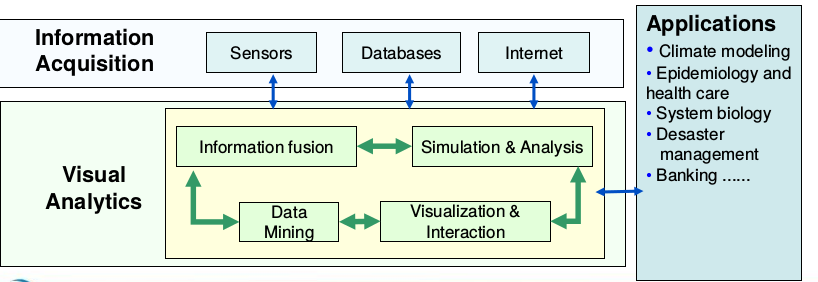
\includegraphics[width=5in]{images/Selection_001.png}\\
	\item The scaleability challenge: information, variables, display, human
	\item Components
	\begin{itemize}
		\item Analytical reasoning
How to maximise human capacity to perceive, understand, and
reason about complex and dynamic data and situations?
\item Visual representations and interaction techniques
How to augment cognitive reasoning with perceptual reasoning
through visual representations and interaction?
\item Data representations and transformations
How to transform data into a representation that is appropriate to
the analytical task and effectively conveys the important content?
\item Production, presentation, and dissemination
How to convey analytical results in meaningful ways to various
audiences? (Also to justify the efforts of visual analytics)
	\end{itemize}
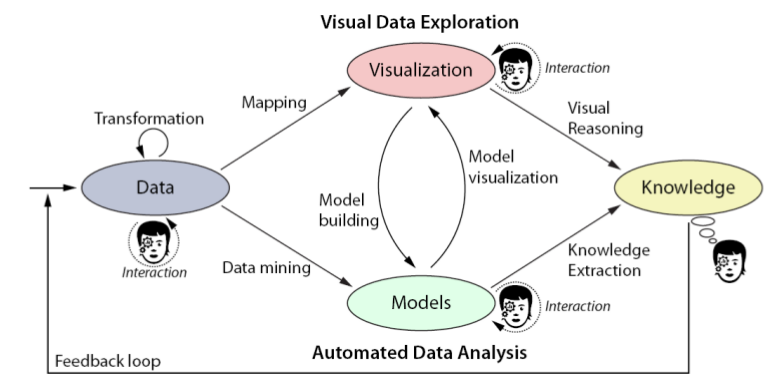
\includegraphics[width=5in]{images/Selection_002.png}\\
	\item Filtering operates on data values and includes
	\begin{itemize}
		\item Data cleansing
		\item Analytical computations, e.g. statistics
	\end{itemize}
	\item reproducible results
	\item Major applications
	\begin{itemize}
		\item Business and finance
		\item Emergency management
		\item Security
		\item Sport analytics
		\item Astronomy
		\item Network analytics
		\item Climate and weather research
	\end{itemize}
\end{itemize}


%%%%%%%%%%%%%%%%%%%%%%%%%%%%%%%%%%%%%%%%%%%%%%%%%%%%%%%%%%%%%%%%

\section{Clustering}

Clustering is part of an exploratory data analysis where users
have little a priori information and serves to define groups automatically (unsupervised
learning).\\

What is clustering good for?
\begin{itemize}
\item Learn the structure of data, e.g. define subgroups for
customer segmentation (business analytics)
\item A preprocess for selective visualization (show only
certain clusters) or for focus-context visualization
(show cluster representatives as overview and all
instances as detailed view)
\item A preprocess for classification, e.g. as input for a
decision tree search
\end{itemize}

According to the model, clustering is performed
\begin{itemize}
\item In a hierarchic or non-hierarchic manner
\item In a fuzzy or binary manner (hard)
\item In a deterministic or non-deterministic manner
\item Using various distance measures
\end{itemize}
Outliers (not belonging to any cluster) are possible with
some approaches.\\
It is easier to interactively merge clusters (right image) than to
separate an erroneously connected cluster.

\subsection{Clustering Methods}
\begin{itemize}
	\item K-Means
\item Optics
\item Density-Based
\item Agglomerative Hierarchical
\item Clustering Ensembles
\end{itemize}

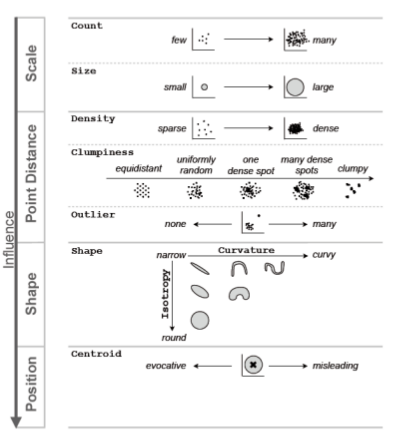
\includegraphics[width=3in]{images/Selection_003.png}
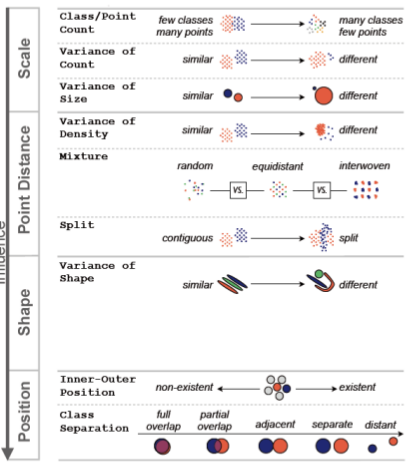
\includegraphics[width=3in]{images/Selection_004.png}

$\rightarrow$ Fuzzy/Hard clustering\\

Clustering may be based on
\begin{itemize}
	\item A distance model
	\item A density model
	\item A hierarchy model where clusters are assumed to
exist at different levels
\end{itemize}

\textbf{k-means}:
\begin{itemize}
	\item Partioning of a dataset in k groups
	\item follows a centroid model (a cluster is defined by its center)
	\item random initialization
	\item convex clusters
	\item not robust
	\item k must be known
	\item not deterministic
\end{itemize}
\textbf{Fuzzy c-means}
\begin{itemize}
 \item With fuzzy clustering objects on the boundaries between
cluster centers are not forced to fully belong to one of them,
but are assigned membership degrees between 0 and 1
indicating partial memberships
\end{itemize}
\textbf{Density base clustering}
\begin{itemize}
	\item do not require an a priori
number of expected clusters and generate clusters
of arbitrary shapes.
	\item Optics and DB-SCAN
	\item Basic concept: density-connectivity $\rightarrow$ two objects are
density connected , if there is a chain of dense objects that
connect the objects
\end{itemize}

\textbf{Hierarchical clustering}
\begin{itemize}
	\item generates a hierarchy of
clustering results
	\item Elements are connected and assigned to a cluster, if
their distance is below a threshold
	\item If the threshold is increased, low level clusters get
connected to higher level clusters
	\item Thus, a hierarchy arises bottom up (agglomerative)
	\item Essential parameters of hierarchical clustering are:
		\begin{itemize}
		\item  Distance function, e.g. Euclidean, Manhattan, Mahalanobis distance
		\item Linkage criterion
		\item The method is not suitable for large element numbers
		\end{itemize}
\end{itemize}

The results of clustering may be improved by with a priori knowledge: Must-link constraints, Cannot-link constraints.\\
Clustering in general is an unsupervised method;
clustering with constraints is supervised

\textbf{Temporal Clustering}



%%%%%%%%%%%%%%%%%%%%%%%%%%%%%%%%%%%%%%%%%%%%%%%%%%%%%%%%%%%%%%%%

\section{Subspace Clustering}

%%%%%%%%%%%%%%%%%%%%%%%%%%%%%%%%%%%%%%%%%%%%%%%%%%%%%%%%%%%%%%%%

\section{Clustering Validation}

%%%%%%%%%%%%%%%%%%%%%%%%%%%%%%%%%%%%%%%%%%%%%%%%%%%%%%%%%%%%%%%%

\section{BiClusters}

%%%%%%%%%%%%%%%%%%%%%%%%%%%%%%%%%%%%%%%%%%%%%%%%%%%%%%%%%%%%%%%%

\section{Scatter plots}

%%%%%%%%%%%%%%%%%%%%%%%%%%%%%%%%%%%%%%%%%%%%%%%%%%%%%%%%%%%%%%%%

\section{Dimension Reduction}

%%%%%%%%%%%%%%%%%%%%%%%%%%%%%%%%%%%%%%%%%%%%%%%%%%%%%%%%%%%%%%%%

\section{Association Rule Mining}

%%%%%%%%%%%%%%%%%%%%%%%%%%%%%%%%%%%%%%%%%%%%%%%%%%%%%%%%%%%%%%%%

\section{Decision Trees}

%%%%%%%%%%%%%%%%%%%%%%%%%%%%%%%%%%%%%%%%%%%%%%%%%%%%%%%%%%%%%%%%

\section{Regression Based Analysis}

%%%%%%%%%%%%%%%%%%%%%%%%%%%%%%%%%%%%%%%%%%%%%%%%%%%%%%%%%%%%%%%%

\section{Temporal Event Sequences}

%%%%%%%%%%%%%%%%%%%%%%%%%%%%%%%%%%%%%%%%%%%%%%%%%%%%%%%%%%%%%%%%

\section{Visual Analytics Healthcare}

%%%%%%%%%%%%%%%%%%%%%%%%%%%%%%%%%%%%%%%%%%%%%%%%%%%%%%%%%%%%%%%%

\section{Interactive cooperative Visual Analytics}

